\chapter{Results and Conclusions}
\label{chap:results}

This chapter outlines the results of the experiments performed with the system using the methods outlined in the preceding chapter. This section is split into two sections. The first section examines the effect of mapping the higher dimensional feature space to a lower dimensional representation using the methods described in section \ref{sec:experiment-features}. The second section presents an investigation into the quality of the mapping.

\section{Comparison of Real and Synthetic Datasets}

For each of the experiments in this section the full set of 360 images of both left, right and mediolateral oblique and craniocaudal views. As the full set of phantoms mammograms represents only a small number of cases (6 in total) if the full set was to be used each phantom would be over represented. To combat features were extracted for all phantoms and then a random phantom was selected from each case to be representative of the case as a whole.

\subsection{Blob features} 

Figure \ref{fig:blob-mapping} shows the result of applying the t-SNE algorithm to the feature matrix of extracted blob radii using the techniques outlined in the methodology to reduce the feature space to two dimensions. Real mammograms are represented by dots and phantom mammograms are represented by triangles. Each data point is coloured by either its BI-RADS risk class (in the case of the reals) or by the volumetric breast density (VBD) (in the case of the phantom mammograms). Figure \ref{fig:blob-mapping3d} shows same features but mapped to 3 dimensions using t-SNE. For both the 2D and 3D cases parameters used for t-SNE were a learning rate of 300 and perplexity of 40.

\begin{figure}
	\label{fig:blob-mapping}
	\centering
	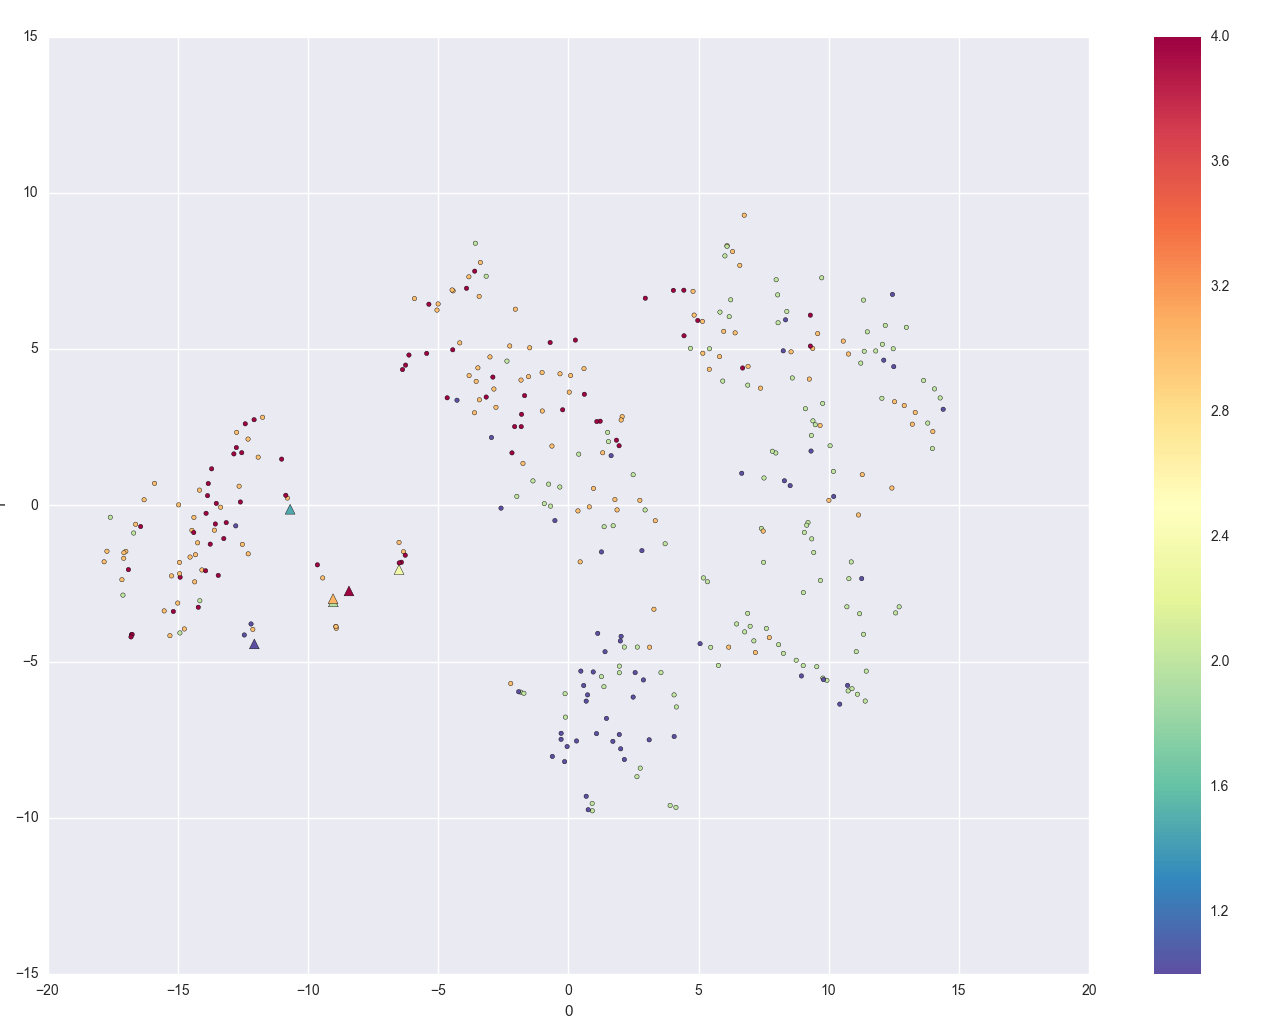
\includegraphics[width=.8\textwidth]{Images/blob-mapping.png}	
	\caption{The 2D visualisation produced by t-SNE from the blob features extracted from real and phantom mammograms. real mammograms are dots and phantoms are triangles.}
\end{figure}

\begin{figure}
	\label{fig:blob-mapping3d}
	\centering
	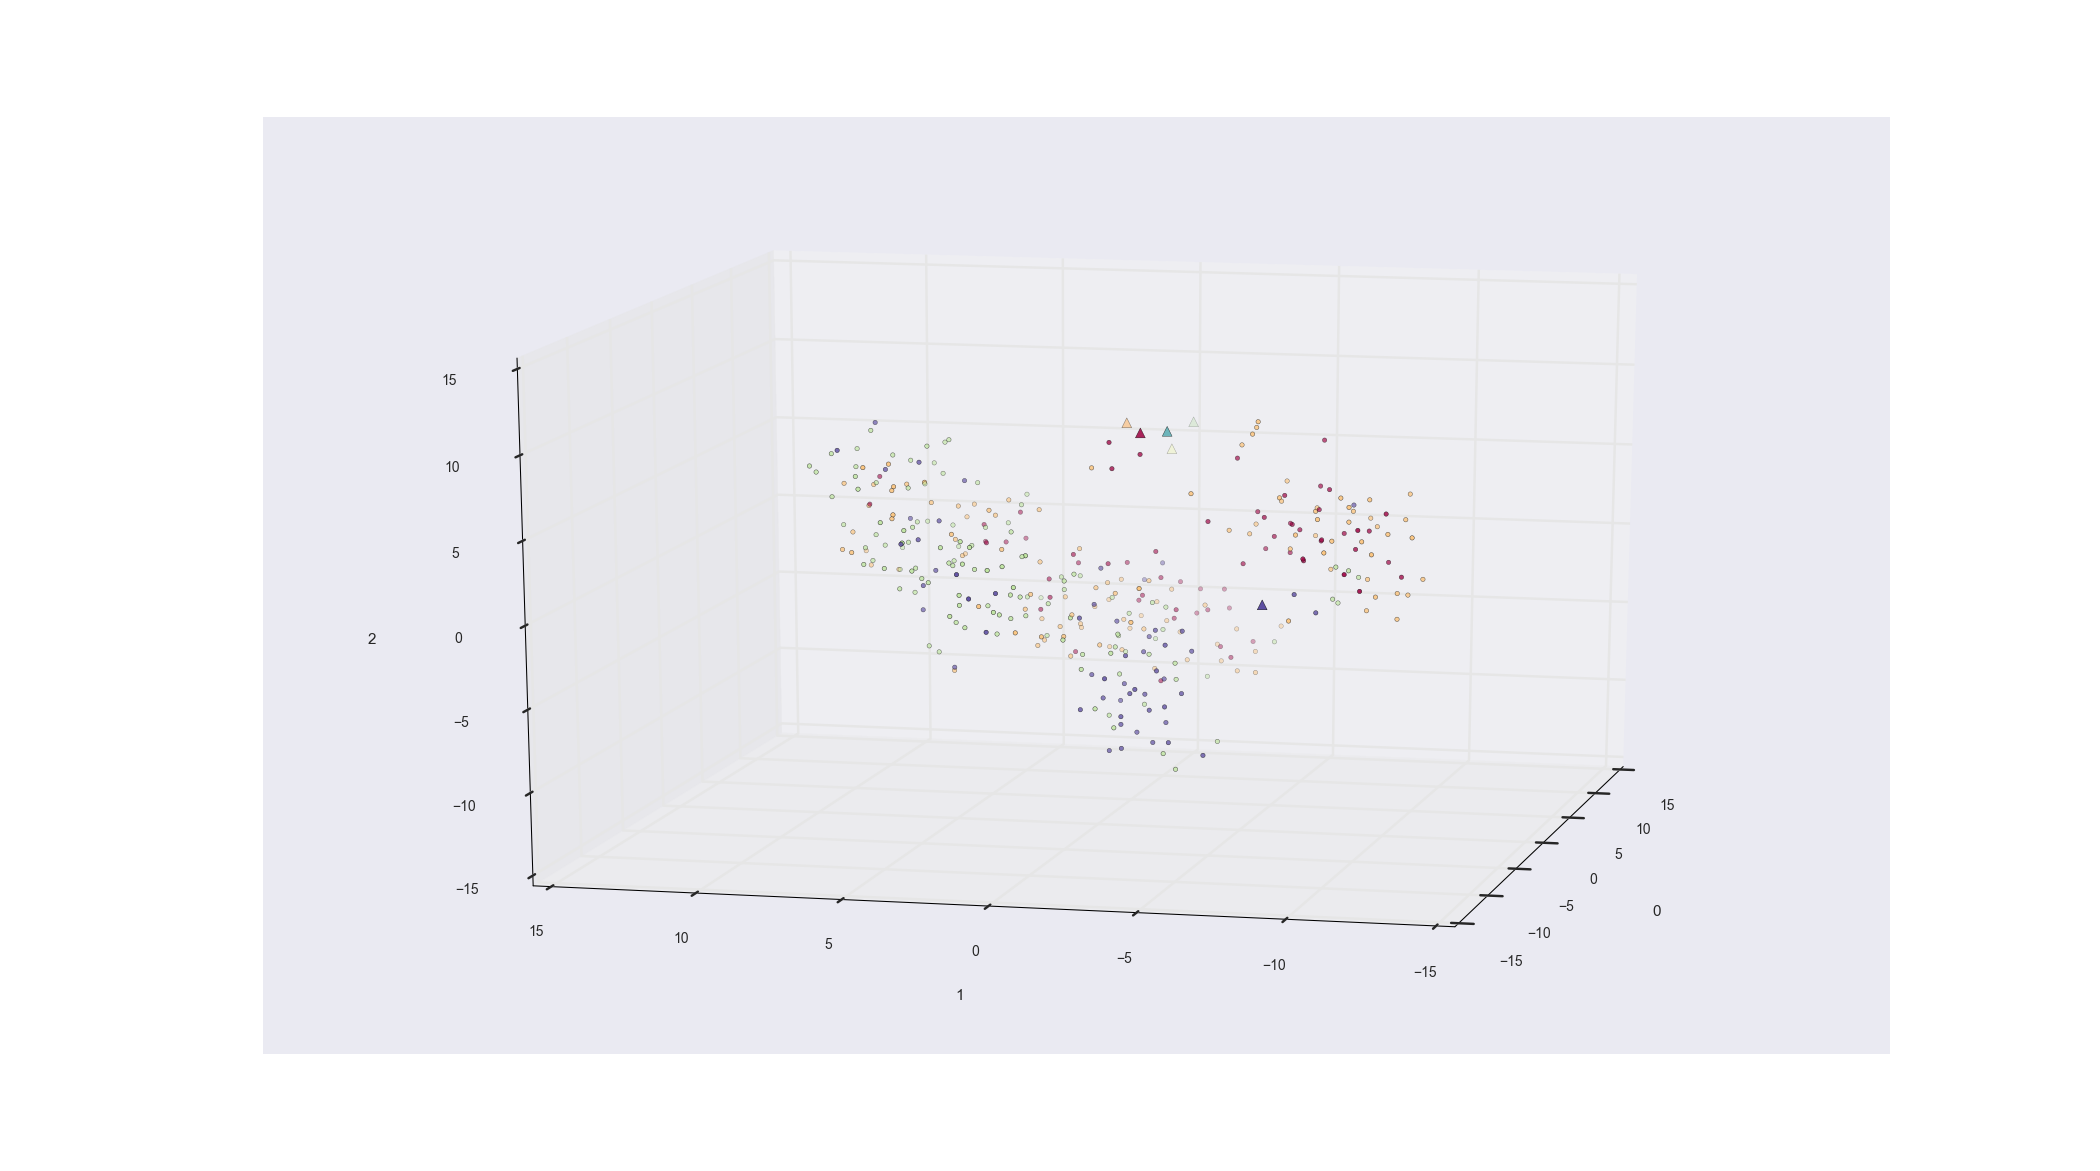
\includegraphics[width=1.0\textwidth]{Images/blob-mapping3d.png}	
	\caption{The 3D visualisation produced by t-SNE from the blob features extracted from real and phantom mammograms. real mammograms are dots and phantoms are triangles.}
\end{figure}

For each of these plots it can be seen that there is some general clustering according to BI-RADS risk class, although separation of risk classes are far from optimum. The distribution of data points shown in figures \ref{fig:blob-mapping} and \ref{fig:blob-mapping3d} are heavily influenced by features relating to the relative proportion of blobs detected across the range of scales. Figure \ref{fig:blob-risk-histogram} shows the number of blobs detected for each scale for each risk class. While the distribution of blobs primarily look the same across all scales, the number of small blobs detected is markedly larger in low risk mammograms.

\begin{figure}[H]
	\label{fig:blob-risk-histogram}
	\centering
	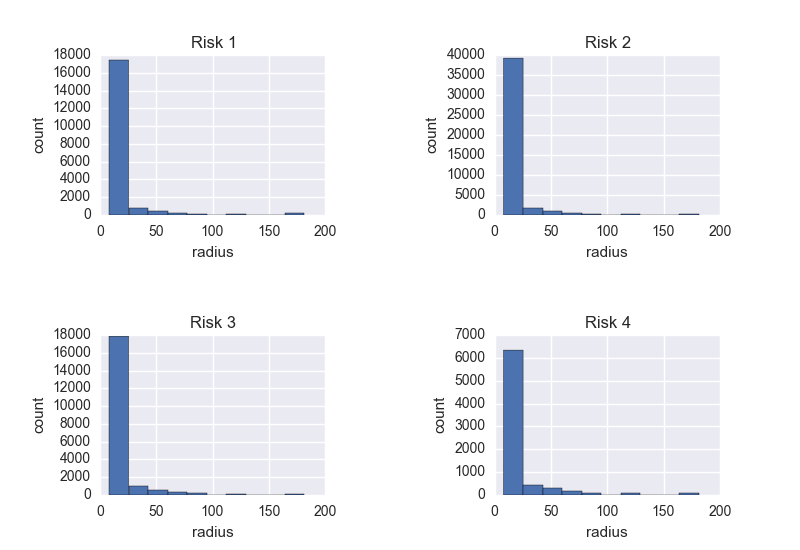
\includegraphics[width=0.8\textwidth]{Images/blob-risk-histogram.png}	
	\caption{Histograms showing the number of blobs at each scale detected across all risk classes for real mammograms.}
\end{figure}

\begin{figure}[H]
	\label{fig:blob-both-dist-avg}
	\centering
	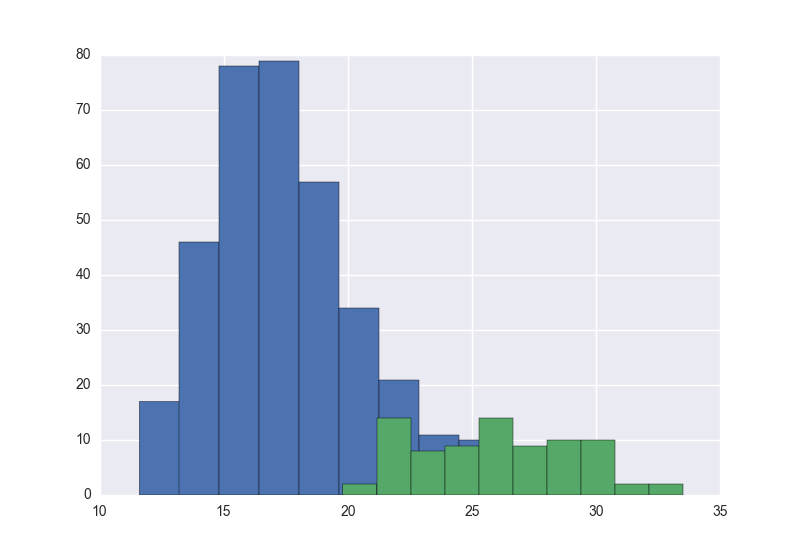
\includegraphics[width=0.7\textwidth]{Images/blob-both-dist-avg.png}	
	\caption{Histograms showing the average blob size for real mammograms (blue) and all phantom mammograms (green)}
\end{figure}

In general the breast phantoms, regardless of the their VBD, are clustered towards mammograms of a higher risk class. This suggests that there are a lower number of smaller blobs present across all VBDs for phantoms. As can be seen from figure \ref{fig:blob-both-dist-avg} the average number of blobs is shifted compared to the real mammograms.


\subsection{Line features}

\subsection{Intensity \& Texture Features}
Texture and intensity features proved proved the least successful for the comparison of the real and phantom datasets. The intensity distribution of the phantom mammograms are nothing like a real mammogram. Because of this difference the results show that the they are clearly in different spaces.

\label{subsec:results-texture}

\section{Quality Evaluation of Mapping}